\documentclass[12pt]{article}

\usepackage[no-math]{fontspec}
\usepackage{polyglossia}
\setdefaultlanguage[
  indentfirst=true,
  spelling=modern]{russian}
\setotherlanguage{english}

\usepackage{amsmath}
\usepackage{unicode-math}
% \usepackage{booktabs}
% \usepackage{array}
% \usepackage{multirow}

\setmainfont{CMU Serif}
\setsansfont{CMU Sans Serif}
\setmonofont{CMU Typewriter Text}

\setmathfont{Latin Modern Math}

\usepackage{cancel}
% \usepackage{latexsym}
\usepackage{hyperref} % ссылки в документе
\hypersetup{
  colorlinks,
  citecolor=black,
  filecolor=black,
  linkcolor=black,
  urlcolor=black,
  bookmarksdepth=subsubsection, 
  unicode=true,       
  pdftoolbar=true,       
  pdfmenubar=true,    
  pdffitwindow=false,  
  pdfstartview={FitH},  
  pdftitle={Черновик о винтовом движении прямой},
  pdfauthor={Коллектив авторов}
}
\usepackage{graphicx} % картинки
\usepackage{xcolor} % цвет


%~~~~~~~~~~~~~~~~~~~~~~~~~~~~~~~~~~~~~~~~~~~~~~~~~~~~~~~~~~~~~~~~~~~~~~~~~~~~~~~
%								BibLaTeX
%~~~~~~~~~~~~~~~~~~~~~~~~~~~~~~~~~~~~~~~~~~~~~~~~~~~~~~~~~~~~~~~~~~~~~~~~~~~~~~~
\usepackage[autostyle]{csquotes}
\usepackage{url}

\usepackage[%
  backend=biber,
  bibstyle=gost-numeric,
  defernumbers=true,
  movenames=false, % не менять местами заголовок и список авторов, если авторов больше четырех
  maxbibnames=10, % сколько авторов указывать
  sorting=none,
]{biblatex}
% Файл с литературой
\addbibresource{bib/algebra.bib}
\addbibresource{bib/zotero/zotero.bib}



%~~~~~~~~~~~~~~~~~~~~~~~~~~~~~~~~~~~~~~~~~~~~~~~~~~~~~~~~~~~~~~~~~~~~~~~~~~~~~~~
%								Theorems
%~~~~~~~~~~~~~~~~~~~~~~~~~~~~~~~~~~~~~~~~~~~~~~~~~~~~~~~~~~~~~~~~~~~~~~~~~~~~~~~
\usepackage[hyperref,thmmarks]{ntheorem}
\theoremseparator{.}
\theoremsymbol{$\mdlgwhtlozenge$}
\theoremheaderfont{\normalfont\bfseries}
\theorembodyfont{\itshape}
\newtheorem{theo}{Теорема}[section]
\theorembodyfont{\normalfont}
\newtheorem{primer}{Пример}
\theoremstyle{nonumberplain}
\theoremheaderfont{\bfseries}
\newtheorem{dokaz}{Доказательство}
\theoremlisttype{allname}

\author{Подмогильный Иван, Дидусь Кирилл, Нельсонович Мигран}
\date{1 марта 2025}
\title{Черновик о винтовом движении прямой}

\begin{document}
  
  \maketitle

  %\tableofcontents
  %\clearpage

  % \subsection{Движение прямой через координаты Плюкера}

  % Книга по алгебре~\cite[Гл. 1 \S 2]{Zulanke:01:2004}. Можно вставить ссылку как сноску, например~\footfullcite{Fedorchuk1990}. Как написано в книге~\fullcite{IlinPosdniak1981}. Ссылка на статью~\cite{PhysRevLett.81.4545} 

  \section{Плюккеровы координаты}

  С помощью Плюккеровых координат (также называемых Грассмановыми координатами) \autocite[Гл. 7]{hodgeMethodsAlgebraicGeometry1994}
  можно задать прямую в трёхмерном проективном пространстве $\mathbb{P}^3$ с помощью шести параметров $\mathbf{L}=(\mathbf{v}:\mathbf{m})=(v_1:v_2:v_3:m_1:m_2:m_3)$.
  Где $\mathbf{v}$ называют направляющим вектором прямой, а $\mathbf{m}$ называют моментом прямой. Координаты направляющего вектора и момента можно представить в виде
  Плюккеровой матрицы: 
  \begin{equation*}
    \mathbf{[L]}_\times = 
    \begin{pmatrix}
      0 & -v_1 & -v_2 & -v_3 \\
      v_1 & 0 & -m_1 & -m_2 \\
      v_2 & m_1 & 0 & m_3 \\
      v_3 & m_2 & m_3 & 0
\end{pmatrix}
  \end{equation*}
  
  \subsection{Движение прямой представленной в Плюккеровых координатах}

  Чтобы подействовать полной линейной группой  GL(3,$\mathbb{R}$) на прямую, можно использовать матрицу преобразования 
  \autocite[Гл. 3.2, секция II. Plücker matrices, пункт 5]{hartley2003multiple}: 

  \begin{equation*}
    \mathbf{H} =
    \begin{pmatrix}
      h_{11} & h_{12} & h_{13} & h_{14} \\
      h_{21} & h_{22} & h_{23} & h_{24} \\
      h_{31} & h_{32} & h_{33} & h_{34} \\
      h_{41} & h_{42} & h_{43} & h_{44} 
  \end{pmatrix}
  \end{equation*}

  Реализацией такого действия будет операция: $[\mathbf{L'}]_\times = \mathbf{HLH^T}$.

  \section{Моторы}

  Ещё одним подходом к представлению прямой являются моторы и винты \autocite{dimentberg1965винтовое}. Чтобы определить мотор, нужно задать дуальный вектор
  - $\{\mathbf{v} \mid \mathbf{m}\}$, в котором как и в Плюккеровых координатах $\mathbf{v}$ - направляющий вектор прямой, $\mathbf{m}$ - момент прямой.
  Мотором называется следующая запись: 
  \begin{equation*}
    R = \{ \mathbf{v} \mid \mathbf{m} \} = \mathbf{v} + \epsilon \mathbf{m}
  \end{equation*}
  Где $\epsilon$ является дуальным числом $\epsilon^2=0$. Напомним, что для дуальных чисел выполняется свойство $\exp{\epsilon x} = 1 + \epsilon x$.
  Изначально дуальные числа были предложены Клиффордом \autocite{cliffordPreliminarySketchBiquaternions1871},
  и в дальнейшем исследованы Штуди \autocite{zindlerGeometrieDynamenStudy1903}

  \subsection{Винты}

  Для любого мотора можно подобрать такую систему координат, что в ней векторы $\mathbf{v}$ и $\mathbf{m}$ будут коллинеарны. 
  Винтом называется мотор, у которого направляющий вектор и момент коллинеарны $\mathbf{m} \| \mathbf{v}$. Винт имеет запись
  \begin{equation*}
    R = \{ \mathbf{v} \mid p\mathbf{v} \} = \mathbf{v} + \epsilon p \mathbf{v} = (1+\epsilon p)\mathbf{v}
  \end{equation*}
  В новой системе координат $p=\frac{(\mathbf{v}, \mathbf{m})}{\| \mathbf{v} \|^2}$ называется параметром винта.
  Винт, у которого норма направляющего вектора равна единице $\| v \| = 1$ называется единичным винтом. Винт можно записать через единичный винт:
  \begin{equation*}
    R = r(1+\epsilon p)\mathbf{E} = r\exp{\epsilon p}\mathbf{E}
  \end{equation*}

  \subsection{Движение прямой через моторы}






  \section{Бикватернионы}

  Кватернионы могут использоваться для выражения поворотов \autocite[Гл. N]{chelnokov2006кватернионные} так как множество единичных кватернионов 
  \begin{equation*}
    S^3 = \{q \in \mathbb{H} \mid \|q\| =1\}
  \end{equation*}
  по произведению Гамильтона даёт группу Ли, которая дважды покрывает специальную ортогональную группу $SO(3)$ \autocite[Гл. 12]{altmann1986rotations}:
  \begin{equation*}
    \phi : S^3 \rightarrow SO(3), \phi(q) = \phi(-q)
  \end{equation*}

  Бикватернионы получаются из кватернионов процедурой Кейли-Диксона (удвоением) и имеют запись:
  \begin{equation*}
    Q = q + \epsilon q^o, \quad q,q^o \in \mathbb{H}, \quad \epsilon^2=0
  \end{equation*}
  Бикватернионы были предложены Клиффордом \autocite{cliffordPreliminarySketchBiquaternions1871}. Более подробно бикватернионы описываются в заметке \autocite{jiaDualQuaternions2018},
  а приложение для свободного движения твёрдого тела (вращение и трансляция) приведено в \autocite[Гл. N]{chelnokov2006кватернионные}

  \subsection{Движение прямой через бикватернионы}

  В алгебре бикватернионов прямая представима в виде чистого бикватерниона: $\mathbf{L} = \mathbf{L}_x i + \mathbf{L}_y j + \mathbf{L}_z k$. Движение и поворот этой
  прямой задается в виде
  \begin{align*}
    &\mathbf{L}' = \mathbf{QLQ^*}, \quad \mathbf{Q} = \Lambda_0 + \Lambda_1 i + \Lambda_2 j + \Lambda_3 k \\
    &\Lambda_0 = cos{\frac{\Theta}{2}}, \Lambda_1 = sin{\frac{\Theta}{2}}A_x, \Lambda_2 = sin{\frac{\Theta}{2}}A_y, \Lambda_3 = sin{\frac{\Theta}{2}}A_z \\
    &\Theta  = \theta + \epsilon \theta^0
  \end{align*}
  Где $\Theta$ называется дуальным углом, а $\mathbf{Q}^*$ сопряженным бикватернионом.

  % Формула может быть в строке $f(x) = \cos{x} + \tg{x} +\ch{x} + \sh{x} + \sin{x} + e^{-\mathrm{i}x}$ еще формула с дробью $\frac{2}{3}$ и еще $\dfrac{2}{3}$

  % \begin{equation}\label{eq:eq01}
  %   f(x) = \sum\limits^{\infty}_{i=0}\frac{x^2 + 1}{x^3 - 1}
  % \end{equation}

  % В формуле~\eqref{eq:eq01} (сравните \verb|\ref{}|~\ref{eq:eq01})

  % \begin{equation*}
  %   F(x) = \int\limits^{\frac{c-b}{d}}_{a}\dfrac{t^2 - t + 1}{\cos{t}}\mathrm{d} t
  % \end{equation*}

  % \begin{equation*}
  %   \mathbf{v} = \vec{v} = 
  %   \begin{pmatrix}
  %     v^1 \\
  %     v^2 \\
  %     v^3
  %   \end{pmatrix}
  %   \quad
  %   \tilde{u} = 
  %   \begin{bmatrix}
  %     u_1 & u_2 & \ldots & u_n 
  %   \end{bmatrix},
  %   \quad
  %   \mathbf{u} = 
  %   \begin{bmatrix}
  %     u^1\\
  %     \vdots\\
  %     u^n
  %   \end{bmatrix}
  % \end{equation*}

  % \begin{equation*}
  %   M = 
  %   \begin{pmatrix}
  %     a^1_1 & a^1_2 & a^1_3\\
  %     a^2_1 & a^2_2 & a^2_3\\
  %     a^3_1 & a^3_2 & a^3_3
  %   \end{pmatrix}
  %   \quad
  %   a = \mathrm{det}\,A = 
  %   \begin{vmatrix}
  %     a^1_1 & \ldots & a^n_1\\
  %     \vdots & \ddots & \vdots\\
  %     a^1_n & \ldots & a^n_n
  %   \end{vmatrix}
  % \end{equation*}

  % \begin{equation*}
  %   \left\{
  %   \begin{aligned}
  %     &x = y,\\
  %     &x = y + x - 1.
  %   \end{aligned}
  %   \right.
  % \end{equation*}

  % \begin{multline}
  %   x^{15} + x^{15} + x^{15} + x^{15} + x^{15} + x^{15} + x^{15} + x^{15} + x^{15} + x^{15} + x^{15} + x^{15} + x^{15} + x^{15} + {}\\
  %   {} + x^{15} + x^{15} + x^{15} + x^{15} + x^{15} + x^{15} + x^{15} + x^{15} + x^{15} + x^{15} + x^{15} + x^{15} + x^{15} + x^{15} + x^{15} + {} \\
  %   {} + x^{15} + x^{15} + x^{15} + x^{15} + x^{15} + x^{15} + 
  % \end{multline}

  % \begin{gather}
  %   x = y\\
  %   x = p + 3\\
  %   \dfrac{1+5}{5+x}\\
  %   \left\{
  %   \begin{aligned}
  %     &x = y,\\
  %     &x = y + x - 1.
  %   \end{aligned}
  %   \right.
  % \end{gather}

  % \begin{equation*}
  %   \langle x_1, x_2 \rangle, \|\mathbf{v}\|
  %   \quad
  %   a \leqslant 0, \quad a \geqslant 0
  % \end{equation*}

  % \begin{equation*}
  %   x \in \mathbb{R}, \quad \mathbb{C} \ni z
  %   \mathbb{Q} \subset \mathbb{R}
  %   \approx, \between, \not=
  % \end{equation*}

  % \begin{equation}
  %   \alpha \beta \rho \varrho \phi \varphi
  %   \Phi, \Delta, \chi, \epsilon, \varepsilon
  %   \Omega_{\alpha}^{\beta}
  %   \varkappa, \kappa
  %   \quad
  %   \alpha
  % \end{equation}

  % \begin{equation*}
  %   \dot{a},\quad
  %   \ddot{a}, \dddot{a}
  %   \quad
  %   \sqrt{x}, \sqrt[3]{x}
  % \end{equation*}

  % \begin{equation*}
  %   \underbrace{a_1 + b_2}_{=0} + \overbrace{c_2 + x(t)}^{\text{что-то написали}} + a - 1 = 0
  % \end{equation*}


  % \begin{equation*}
  %   \cancel{a_1} + \bcancel{b_2} + \xcancel{c_2} +
  %   \cancelto{0}{x(t)} + a - 1 = 0
  % \end{equation*}

  % \begin{equation}
  %   \mathbf{v}, \vec{v}, \hat{j}, \Vec{j}, \vec{j}
  % \end{equation}

  % \begin{equation*}
  %   \left( \dfrac{\sum^{\infty}_{i=0}{\dfrac{x_i + 1}{x_i - 1}}}{\int\limits^{+\infty}_{-\infty}f(x)\mathrm{d} x} \right)
  % \end{equation*}

  % \begin{equation}
  %   \big( x \Big)
  % \end{equation}


  % \begin{equation*}
  %   \lim_{x \to 0}\dfrac{x^2 + 1}{x^2 - 1}
  % \end{equation*}

  % \begin{equation*}
  %   x^{i\to 0} \Leftrightarrow y^{t \leftarrow 0}
  % \end{equation*}

  % \begin{equation*}
  %   y = \Im{z} \quad x = \Re{z} 
  % \end{equation*}

  % \begin{equation*}
  %   x^{\dag}
  % \end{equation*}

  % \begin{equation*}
  %   \overline{a + b}
  % \end{equation*}

  % \begin{equation*}
  %   C^{k}_{n} = \binom{k}{n}
  % \end{equation*}

  % \begin{equation*}
  %   \tg{x} \quad tg{x}
  %   \sinh \quad \sh
  % \end{equation*}

  \begin{equation*}
    \mathbb{R}
    \quad
    R \;\; \mathtt{R}
    \quad
    \mathcal{R} \quad \mathfrak{R} \mathfrak{G} \mathfrak{S}\mathfrak{L}\mathfrak{K}
  \end{equation*}

  % Внутри \texttt{абзаца} \(x + 1 = 9\)

  \section{Геометрическая алгебра}

  \subsection{Элементы теории групп}

  \subsection{Движение прямой через геометрическую алгебру}
  
% \autocite{bayro-corrochanoSurveyQuaternionAlgebra2021}

  % \subsection{Факт №1}

  % A \emph{bulletproof} vest wears Chuck Norris for protection.
  % If Chuck Norris were to travel to an alternate dimension 
  % in which there was another Chuck \emph{Norris} and they both 
  % fought, they would both win. It takes Chuck Norris 
  % 20 minutes        to watch 60 Minutes. Chuck Norris once 
  % shattered the space-time \textbf{continuum}. He felt so bad, 
  % he put it back together. \textit{Chuck Norris} can 
  % sit in the corner of a round room.

  % \subsubsection{Подфакт о Чаке Норрисе}

  % If it looks like chicken, tastes like chicken, and feels like chicken but Chuck Norris says its beef, then it’s beef. Chuck Norris knows Victoria’s secret. Chuck Norris is the reason why Waldo is hiding. When Chuck Norris does a pushup, he’s pushing the Earth down. Chuck Norris invented airplanes because he was tired of being the only person that could fly.

  % Не нумерованный список.
  % \begin{itemize}
  %   \item Пункт номер 1
  %   \item Пункт номер 2
  %   \item Пункт номер 3
  %   на нескольких строках
  %   вполне можно это сделать
  % \end{itemize}

  % Нумерованный список.
  % \begin{enumerate}
  %   \item Пункт номер 1
  %   \item The Great Wall of China was originally created to keep Chuck Norris out. It didn’t work.
  %   \item When Christopher Columbus discovered America, he was greeted by Chuck Norris.
  % \end{enumerate}

  % \begin{description}
  %   \item[№1] Раз
  %   \item[№2] Два
  %   \item[№3] Три Chuck Norris once ordered a steak in a restaurant. The steak did what it was told. Chuck Norris can squeeze orange juice out of a lemon.

  % \end{description}

  % \begin{figure}[h!]
  %   \center
  %   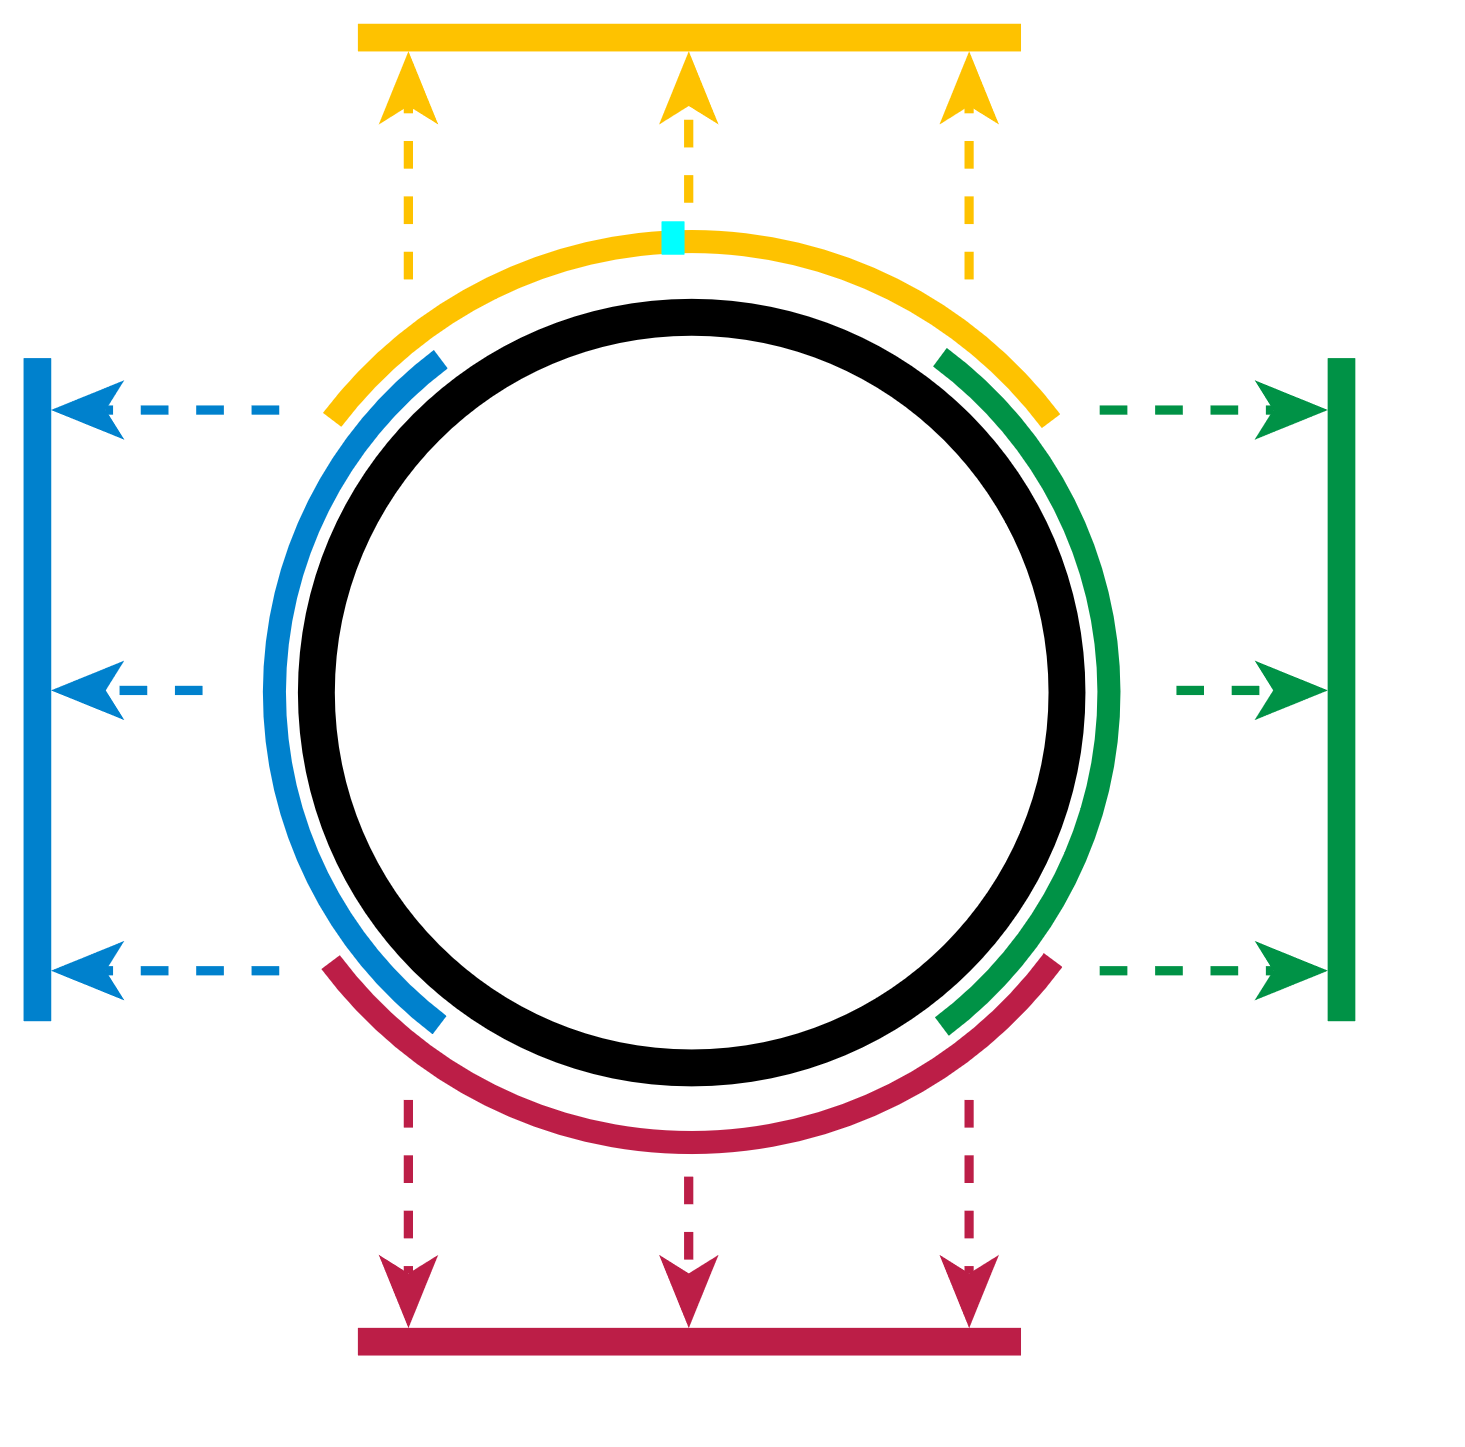
\includegraphics[width=0.5\textwidth]{img/circle.png}
  %   \caption{Подпись к картинке}
  %   \label{fig:img01}
  % \end{figure}

  % Chuck Norris sleeps with a pillow under his gun. Chuck Norris used to beat the shit out of his shadow because it was following to close. It now stands a safe 30 feet behind him. Look at fig.~\ref{fig:img01}. Chuck refers to himself in the fourth person. Chuck Norris once shattered the space-time continuum. He felt so bad, he put it back together. Chuck Norris has never blinked in his entire life. Never.

  

  % \begin{verbatim}
  %   #include <stdio.h>

  %   int main() {
  %     return 0;
  %   }
  % \end{verbatim}

  % Какой-то текст на русском языке.


  \printbibliography
  
\end{document}

